% Preamble {{{
\documentclass[]{beamer}
\usepackage{ngerman}

\providecommand\thispdfpagelabel[1]{}

\usepackage[utf8]{inputenc}
%\usepackage[T1]{fontenc}
\usepackage{cite}

\usepackage{verbatim}

\usepackage{amssymb}

\usepackage{tikz}
\usetikzlibrary{shapes,fadings}

\usepackage{hyperref}

\tikzstyle{blob}=[rectangle,
	thick,
	minimum size=0.8cm,
	draw=purple!80,
	fill=purple!20]

\tikzstyle{tree}=[rectangle,
	thick,
	minimum size=0.8cm,
	draw=blue!80,
	fill=blue!20]

\tikzstyle{commit}=[rectangle,
	thick,
	minimum size=0.8cm,
	draw=green!80,
	fill=green!20]

\tikzstyle{branch}=[rectangle,
	thick,
	minimum size=0.8cm,
	draw=yellow!80,
	fill=yellow!20]

\tikzstyle{tag}=[rectangle,
	thick,
	minimum size=0.8cm,
	draw=orange!80,
	fill=orange!20]

% Preamble }}}
%\definecolor{OneFg}{RGB}{0,0,0}
%\definecolor{OneBg}{RGB}{161,255,135}
%\definecolor{TwoFg}{RGB}{0,0,0}
%\definecolor{TwoBg}{RGB}{9,249,198}
%\definecolor{ThreeFg}{RGB}{0,0,0}
%\definecolor{ThreeBg}{RGB}{255,107,33}
%\definecolor{FourFg}{RGB}{255,255,255}
%\definecolor{FourBg}{RGB}{239,163,122}
%\definecolor{FiveFg}{RGB}{0,0,0}
%\definecolor{FiveBg}{RGB}{177,229,237}

\definecolor{OneFg}{RGB}{0,0,0}
\definecolor{OneBg}{RGB}{209,242,165}
\definecolor{TwoFg}{RGB}{0,0,0}
\definecolor{TwoBg}{RGB}{239,250,180}
\definecolor{ThreeFg}{RGB}{0,0,0}
\definecolor{ThreeBg}{RGB}{255,196,140}
\definecolor{FourFg}{RGB}{0,0,0}
\definecolor{FourBg}{RGB}{255,159,128}
\definecolor{FiveFg}{RGB}{0,0,0}
\definecolor{FiveBg}{RGB}{245,105,145}

\definecolor{FooFg}{RGB}{84,36,55}
\definecolor{FooBg}{RGB}{250,211,178}

\definecolor{Christian}{RGB}{0,102,204}

% \usebackgroundtemplate{
% 	\includegraphics[width=\paperwidth, height=\paperheight]{foo.pdf}
% }
\newcommand{\normalstyle}{
	\setbeamercolor{background canvas}{bg=}
	\setbeamercolor{frametitle}{fg=FooFg}
}

\newcommand{\styleFoo}{
	\setbeamercolor{background canvas}{bg=FooBg}
	\setbeamercolor{frametitle}{fg=FooFg}
}

\newcommand{\styleOne}{
	\setbeamercolor{background canvas}{bg=OneBg}
	\setbeamercolor{frametitle}{fg=OneFg}
}

\subject{Version Control -- eine Einführun}

\newcommand{\todo}{\textcolor{red}{\textbf{ \textsf{TODO} }}\\}


\begin{document}
\setbeamercolor{frametitle}{fg=Christian}
\setbeamercolor{framesubtitle}{fg=Christian}
\setbeamercolor{item}{fg=Christian}

\title[Version Control]{Version Control -- eine Einführung}
\subtitle[Zoran Zari\'c]{Zoran Zari\'c}
\author[Zoran Zari\'c]{Zoran Zari\'c}

\begin{frame}
	\fontsize{30}{10}\selectfont Version Control
	\vspace*{0.5cm}

	\fontsize{20}{10}\selectfont eine Einführung
\end{frame}

\begin{frame}
	\frametitle{Zoran Zari\'c}
	\begin{itemize}
		\item
			2007 Ausbildung zum Fachinformatiker für Systemintegration
		\item
			Informatik Student an der TU Darmstadt seit 2008
		\item
			Git seit Mitte 2009
		\item
			bup seit April 2010
	\end{itemize}
\end{frame}

\begin{frame}
	\frametitle{toc}
	\begin{enumerate}
		\item
			Fragen
		\item
			Basics
		\item
			Git
		\item
			Beispiele / Demo
		\item
			Hintergründe
		\item
			Tools
	\end{enumerate}
\end{frame}

\section{Fragen}
\begin{frame}
	\fontsize{30}{10}\selectfont Fragen
\end{frame}

\begin{frame}
	\frametitle{Fragen}
	\begin{enumerate}
		\item<1->
			Wer weiß was Version Control ist?
		\item<2->
			Wer kennt Subversion / CVS?
		\item<3->
			Wer weiß was \emph{Distributed} Version Control ist?
		\item<4->
			Wer kennt Git / Mercurial?

	\end{enumerate}
\end{frame}

\begin{frame}
	\frametitle{Fragen}
	\Huge{Version Control?}\\
\end{frame}

\begin{frame}[fragile]
	\frametitle{Fragen}
	\begin{verbatim}
	$ echo "Halo Wlet!" > README
	\end{verbatim}

	\begin{verbatim}
	$ mkdir v0.1
	$ mv README v0.1
	\end{verbatim}

	\begin{verbatim}
	$ echo "Hallo Welt!" > README
	\end{verbatim}
\end{frame}

\begin{frame}
	\frametitle{Fragen}
	\Huge{\emph{Distributed} Version Control?}
\end{frame}

\begin{frame}[fragile]
	\frametitle{Fragen}
	\begin{verbatim}
		$ echo "Hier die bestimmt finale Version unseres Codes" \ 
		| mail -s "Code final, echt jetzt" -a main.c foo@bar.com
	\end{verbatim}
\end{frame}

\subsection{Git}
\begin{frame}
	\frametitle{Git}
	\begin{itemize}
		\item
			``stupid content tracker''
		\item
			``content addressable''
		\item
			Verteiltes Versionierungssystem
			\begin{itemize}
				\item
					Vollständige Kopie des Repositories lokal
				\item
					lokales Committen, Branchen, Mergen
			\end{itemize}
		\item
			Linus Torvalds begann Entwicklung 2005
		\item
			Snapshot- statt Diff-basiert
	\end{itemize}
\end{frame}

\begin{frame}
	\frametitle{Fragen}
	\Huge{Diffs? Snapshots?}
\end{frame}

\begin{frame}[fragile]
	\frametitle{Fragen}
	\framesubtitle{Diffs? Snapshots?}
	\begin{columns}[T]
		\begin{column}{4.5cm}
		\huge{Diffs} \normalsize (Subversion)

		\begin{verbatim}
		$ cat foo.1
		Halo Wlet!

		$cat foo.2.diff
		1c1
		< Halo Wlet!
		---
		> Hallo Welt!

		$patch foo.1 -o - < foo.2.diff
		patching file foo.1
		Hallo Welt!
		\end{verbatim}
		\end{column}

		\begin{column}{4.5cm}
		\huge{Snapshots} \normalsize (Git)

		\begin{verbatim}
		$ cat foo.1
		Halo Wlet!

		$cat foo.2
		Hallo Welt!
		\end{verbatim}
		\end{column}
	\end{columns}
\end{frame}

\subsection{Installation}
\begin{frame}[fragile]
	\frametitle{Installation}
	\begin{itemize}
		\item
			Windows\\
			mysysgit \url{http://code.google.com/p/msysgit/}\\
			TortoiseGit \url{http://code.google.com/p/tortoisegit/}
		\item
			Ubuntu\\
			\verb|aptitude install git|
		\item
			OSX\\
			\url{http://code.google.com/p/git-osx-installer/}
	\end{itemize}
\end{frame}

\subsection{Beispiel}
\begin{frame}[fragile]
	\frametitle{Beispiele}
	\framesubtitle{Config}
	\begin{verbatim}
	$ git config user.name "Zoran Zaric"
	$ git config user.email "zz@zoranzaric.de"
	\end{verbatim}
\end{frame}

\begin{frame}[fragile]
	\frametitle{Beispiele}
	\framesubtitle{Erste Schritte}
	\begin{columns}[T]
		\begin{column}{7.5cm}
			\begin{verbatim}
			$ git init
			\end{verbatim}

			\begin{verbatim}
			$ echo "Halo Wlet!" > README
			$ git add README
			$ git commit -m "Initial import" # (1)
			\end{verbatim}

			\begin{verbatim}
			$ git log
			\end{verbatim}

			\begin{verbatim}
			$ echo "Hallo Welt!" > README
			$ git add README
			$ git commit -m "Fix spelling errors" # (2)
			\end{verbatim}

			\begin{verbatim}
			$ git log
			\end{verbatim}
		\end{column}
		\begin{column}{2.5cm}
			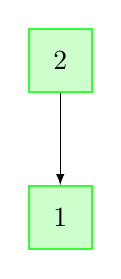
\begin{tikzpicture}
				\node[circle] (b) [commit]{2};
				\node[circle] (a) [commit, below of=b, node distance=2cm]{1};
				\draw[-latex] (b) -- (a);
			\end{tikzpicture}
		\end{column}
	\end{columns}
\end{frame}

\begin{frame}[fragile]
	\frametitle{Beispiele}
	\framesubtitle{Branchen und Mergen}
	\begin{columns}[T]
		\begin{column}{7.5cm}
			\begin{verbatim}
			$ git status
			# On branch master
			\end{verbatim}

			\begin{verbatim}
			$ git checkout -b new-branch
			$ git branch
			\end{verbatim}

			\begin{verbatim}
			$ echo "Lorem ipsum" >> README
			$ git add README
			$ commit -m "Add noise" # (3)
			\end{verbatim}

			\begin{verbatim}
			$ git diff master
			$ git checkout master
			$ git merge new-branch
			$ git branch -d new-branch
			\end{verbatim}
		\end{column}
		\begin{column}{2.5cm}
			\begin{tikzpicture}
				\node[circle] (a) [commit, above right of=b, node distance=2cm]{3};
				\node[circle] (b) [commit]{2};
				\node[circle] (c) [commit, below of=b, node distance=2cm]{1};
				\draw[-latex] (b) -- (c);
				\draw[-latex] (a) -- (b);
			\end{tikzpicture}
		\end{column}
	\end{columns}
\end{frame}

\begin{frame}
	\fontsize{30}{10}\selectfont Äääähm!
	\vspace*{0.5cm}

	\fontsize{20}{10}\selectfont war da nicht was mit \emph{distributed}?!1elf
\end{frame}

\begin{frame}[fragile]
	\frametitle{Beispiele}
	\framesubtitle{Remotes}
	\begin{verbatim}
	$ git clone https://github.com/apenwarr/bup.git
	$ git remote rename origin upstream
	\end{verbatim}

	\begin{verbatim}
	# Änderungen holen
	$ git fetch upstream
	$ git merge upstream/master
	\end{verbatim}

	\begin{verbatim}
	# Änderungen hochladen
	$ git push upstream master
	\end{verbatim}
\end{frame}

\begin{frame}
	\fontsize{30}{10}\selectfont Aber, aber\ldots
	\vspace*{0.5cm}

	\fontsize{20}{10}\selectfont upstream sind Änderungen und ich habe
	Änderungen\ldots\ und\ldots\ und\ldots\ jetzt?
\end{frame}

\begin{frame}[fragile]
	\frametitle{Beispiele}
	\framesubtitle{Rebase}
	\begin{columns}[T]
		\begin{column}{7.5cm}
			\begin{verbatim}
			# Lokale Änderungen auf Basis
			# von upstream/master
			$ echo "..." >> README
			$ git add README
			$ git commit -m "..." # (3)
			\end{verbatim}

			\begin{verbatim}
			# Änderungen holen
			$ git fetch upstream # (4)
			\end{verbatim}
		\end{column}
		\begin{column}{2.5cm}
			\begin{tikzpicture}
				\node[circle] (a1) [commit, above of=b, node distance=2cm]{4};
				\node[circle] (a2) [commit, above right of=b, node distance=2cm]{3};
				\node[circle] (b) [commit]{2};
				\node[circle] (c) [commit, below of=b, node distance=2cm]{1};
				\draw[-latex] (b) -- (c);
				\draw[-latex] (a1) -- (b);
				\draw[-latex] (a2) -- (b);
			\end{tikzpicture}
		\end{column}
	\end{columns}
\end{frame}

\begin{frame}[fragile]
	\frametitle{Beispiele}
	\framesubtitle{Rebase}
	\begin{columns}[T]
		\begin{column}{7.5cm}
			\begin{verbatim}
			# Lokale Änderungen auf Basis
			# von upstream/master
			$ echo "..." >> README
			$ git add README
			$ git commit -m "..." # (3)
			\end{verbatim}

			\begin{verbatim}
			# Änderungen holen
			$ git fetch upstream # (4)
			\end{verbatim}

			\begin{verbatim}
			# Eigene Änderungen auf Upstream
			# anwenden
			$ git rebase upstream/master
			\end{verbatim}
		\end{column}
		\begin{column}{2.5cm}
			\begin{tikzpicture}
				\node[circle] (a1) [commit, above of=b, node distance=2cm]{4};
				\node[circle] (a2) [commit, above right of=a1, node distance=2cm]{3};
				\node[circle] (b) [commit]{2};
				\node[circle] (c) [commit, below of=b, node distance=2cm]{1};
				\draw[-latex] (b) -- (c);
				\draw[-latex] (a1) -- (b);
				\draw[-latex] (a2) -- (a1);
			\end{tikzpicture}
		\end{column}
	\end{columns}
\end{frame}

\section{Hintergründe}
\begin{frame}
	\frametitle{Basics}
	\begin{itemize}
		\item
			SHA1
		\item
			DAG (Directed Acyclic Graph)\\
			gerichteter zyklenfreier Graph
	\end{itemize}
\end{frame}

\begin{frame}[fragile]
	\frametitle{Ein Repository}
	\begin{columns}[T]
		\begin{column}{4.5cm}
			\begin{itemize}
				\item<1->
					BLOBs\\[0.25cm]
					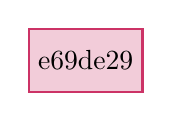
\begin{tikzpicture}
						\node (e69de29) [blob]{e69de29};
					\end{tikzpicture}
				\item<2->
					Trees\\[0.25cm]
					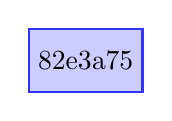
\begin{tikzpicture}
						\node (82e3a75) [tree]{82e3a75};
					\end{tikzpicture}
				\item<3->
					Commits\\[0.25cm]
					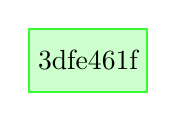
\begin{tikzpicture}
						\node (3dfe461f) [commit]{3dfe461f};
					\end{tikzpicture}
				\item<4->
					Tags \& Branches\\[0.25cm]
					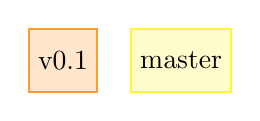
\begin{tikzpicture}
						\node (v01) [tag]{v0.1};
						\node (master) [branch, right of=v01, node distance=1.5cm]{master};
					\end{tikzpicture}
			\end{itemize}
		\end{column}
		\begin{column}{5.5cm}
			\only<1>{
				Hello World
			}
			\only<2>{
				100644 blob 5e1c309dae7f45e0f39b1bf3ac3cd9db12e7d689    README
			}
			\only<3>{
				tree a3d703e579dc9baae20456eb63fa49f5e4e7c9b4\\
				author Zoran Zaric \textless zz@zoranzaric.de\textgreater 1314498536 +0200\\
				committer Zoran Zaric \textless zz@zoranzaric.de\textgreater 1314498536 +0200\\

				Example commit
			}
			\only<5>{
				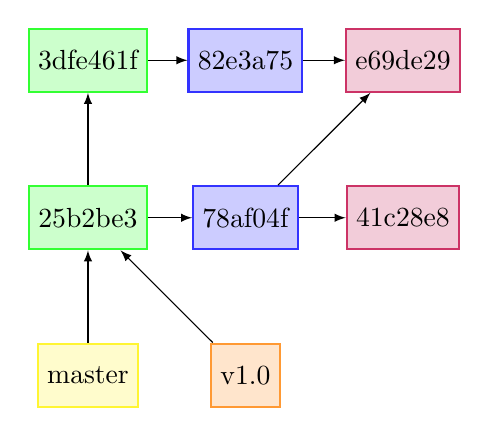
\begin{tikzpicture}
					\node (3dfe461f) [commit]{3dfe461f};
					\node (82e3a75) [tree, right of=3dfe461f, node distance=2cm]{82e3a75};
					\draw[-latex] (3dfe461f) -- (82e3a75);
					\node (e69de29) [blob, right of=82e3a75, node distance=2cm]{e69de29};
					\draw[-latex] (82e3a75) -- (e69de29);

					\node (25b2be3) [commit, below of=3dfe461f, node distance=2cm]{25b2be3};
					\draw[-latex] (25b2be3) -- (3dfe461f);
					\node (78af04f) [tree, right of=25b2be3, node distance=2cm]{78af04f};
					\draw[-latex] (25b2be3) -- (78af04f);
					\draw[-latex] (78af04f) -- (e69de29);
					\node (41c28e8) [blob, right of=78af04f, node distance=2cm]{41c28e8};
					\draw[-latex] (78af04f) -- (41c28e8);

					\node (master) [branch, below of=25b2be3, node distance=2cm]{master};
					\draw[-latex] (master) -- (25b2be3);

					\node (v10) [tag, right of=master, node distance=2cm]{v1.0};
					\draw[-latex] (v10) -- (25b2be3);
				\end{tikzpicture}
			}
		\end{column}
	\end{columns}
\end{frame}

\begin{frame}
	\frametitle{Ein Repository}
	\begin{columns}[T]
		\begin{column}{4.5cm}
			\begin{itemize}
				\item
					DAG\\ Directed Acyclic Graph
				\item<2->
					Packfiles
			\end{itemize}
		\end{column}
		\begin{column}{5.5cm}
			\only<1>{
				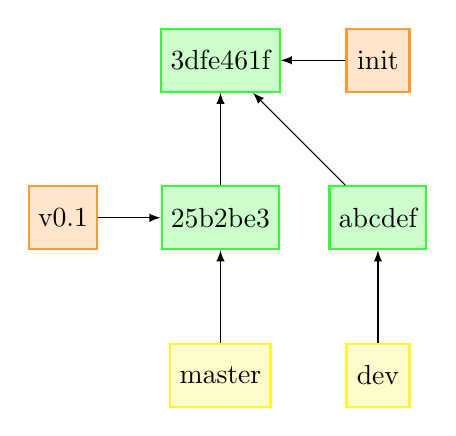
\begin{tikzpicture}
					\node (3dfe461f) [commit]{3dfe461f};
					\node (init) [tag, right of=3dfe461f, node distance=2cm]{init};
					\draw[-latex] (init) -- (3dfe461f);
					\node (25b2be3) [commit, below of=3dfe461f, node distance=2cm]{25b2be3};
					\draw[-latex] (25b2be3) -- (3dfe461f);
					\node (master) [branch, below of=25b2be3, node distance=2cm]{master};
					\draw[-latex] (master) -- (25b2be3);
					\node (v01) [tag, left of=25b2be3, node distance=2cm]{v0.1};
					\draw[-latex] (v01) -- (25b2be3);

					\node (abcdef) [commit, right of=25b2be3, node distance=2cm]{abcdef};
					\draw[-latex] (abcdef) -- (3dfe461f);
					\node (dev) [branch, below of=abcdef, node distance=2cm]{dev};
					\draw[-latex] (dev) -- (abcdef);
				\end{tikzpicture}
			}
			\only<2>{
				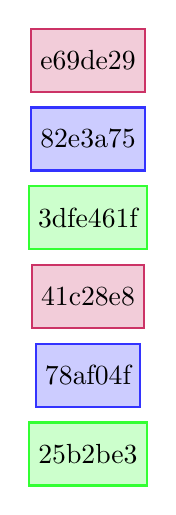
\begin{tikzpicture}
					\node (e69de29) [blob]{e69de29};
					\node (82e3a75) [tree, below of=e69de29]{82e3a75};
					\node (3dfe461f) [commit, below of=82e3a75]{3dfe461f};

					\node (41c28e8) [blob, below of=3dfe461f]{41c28e8};
					\node (78af04f) [tree, below of=41c28e8]{78af04f};
					\node (25b2be3) [commit, below of=78af04f]{25b2be3};
				\end{tikzpicture}
			}
		\end{column}
	\end{columns}
\end{frame}

\section{Tools}
\begin{frame}
	\fontsize{30}{10}\selectfont Tools
\end{frame}

\begin{frame}
	\frametitle{Tools}
	\begin{itemize}
		\item
			Tig
		\item
			gitk
		\item
			gitg
		\item
			Tower Git
		\item
			gitkx
	\end{itemize}
\end{frame}

\begin{frame}
	\frametitle{Weiterführendes / Nachschlagewerk}
	\begin{itemize}
		\item
			\url{http://progit.org/}
		\item
			\url{http://gitref.org/}
		\item
			\url{http://sea.ucar.edu/event/unlocking-secrets-git}
		\item
			\url{http://blip.tv/scott-chacon}
	\end{itemize}
\end{frame}

\begin{frame}[fragile]
	\frametitle{Danke}
	\begin{itemize}
		\item
			\verb|zorzar| auf freenode \& hackint
		\item
			zz@zoranzaric.de (Email \& Jabber)
		\item
			\url{zoranzaric.de}
		\item
			\url{github.com/zoranzaric}
		\item
			\url{gplus.zoranzaric.de}
		\item
			@zoranzaric\\[0.5cm]
		\item
			Slides: \url{zoranzaric.de/git-ophase1112.pdf}
	\end{itemize}
\end{frame}

\end{document}
